\documentclass{aip-cp}

\usepackage[numbers]{natbib}
\usepackage{rotating}
\usepackage{graphicx}
\usepackage{subcaption}

% \usepackage{amsmath,amsthm} 
% \usepackage{amsfonts}
% \usepackage{auto-pst-pdf} 

%\makeatletter
%\def\@fnsymbol#1{\ensuremath{\ifcase#1\or *\or \dagger\or **\or
%   \ddagger\or \mathsection\or \mathparagraph\or \|\or \dagger\dagger
%   \or \ddagger\ddagger \or\mathsection\mathsection
%   \or \mathparagraph\mathparagraph \or *{*}*\or
%   \dagger{\dagger}\dagger \or\ddagger{\ddagger}\ddagger\or
%   \mathsection{\mathsection}\mathsection
%   \or \mathparagraph{\mathparagraph}\mathparagraph \else\@ctrerr\fi}}
%\makeatother

% Document starts
\begin{document}

% Title portion
\title{Investigation on Minimal Hamiltonian for System of Material with Highly Anisotropic Transport and Optical Properties}

% \author[aff1]{Bayu Aditya\noteref{note1,note2}}
\author[aff1]{Bayu Aditya}
\eaddress[url]{http://www.aip.org}
\eaddress{bayu.aditya@sci.ui.ac.id}
\author[aff1]{Muhammad Aziz Majidi\corref{cor1}}

\affil[aff1]{Department of Physics, Faculty of Mathematics and Natural Sciences, Universitas Indonesia, Kampus UI Depok, Indonesia}
\corresp[cor1]{Corresponding author: aziz.majidi@sci.ui.ac.id}
% \authornote[note1]{This is an example of first authornote.}
% \authornote[note2]{This is an example of second authornote.}

\maketitle


\begin{abstract}
Pada penelitian di Departemen Fisika, National University Singapore (NUS) terhadap material Sr1-yNbO3+delta mengungkapkan bahwa material tersebut memiliki karakteristik anisotropik yang sangat tinggi, yaitu bersifat konduktor di sumbu kristal a, dan bersifat insulator di sumbu kristal b dan c. Hal tersebut terjadi karena adanya kontribusi dari orbital pada atom tertentu yang membuat material tersebut bersifat anisotropik. Untuk mengetahui orbital yang berkontribusi tersebut, kami merekonstruksi hamiltonian Tight-Binding multiband dan mereduksi orbital-orbital yang berdampak lemah pada daerah sekitar fermi level, sehingga akan didapat hamiltonian minimal yang memiliki karakteristik anisotropik. Hasil menunjukkan bahwa orbital-d pada atom Nb tertentu, atom O yang berada di antara Nb dan struktur kristal $\mathrm{SrNbO_{3,4}}$ itu sendiri yang memiliki konstribusi pada material sehingga bersifat anisotropik.
\end{abstract}

% Head 1
\section{INTRODUCTION}
Strontium Niobates dengan tipe $\mathrm{SrNbO_{3.4}}$ memiliki hal yang menarik untuk diteliti karena struktur dan properti fisiknya\cite{andrivo}. Material $\mathrm{SrNbO_{3.4}}$ merupakan turunan dari senyawa $\mathrm{SrNbO_{3}}$ dengan adanya tambahan oksigen, dipisahkan dengan oktahedra $\mathrm{NbO_{6}}$ di arah bidang $\{110\}$ \cite{LICHTENBERG2001,LICHTENBERG2008}. Karena adanya tambahan oksigen, maka material tersebut membentuk suatu antarmuka yang sangat mempengaruhi pengisian elektron Nb di orbital-d.\cite{chen}.

Penelitian sebelumnya mengungkapkan bahwa material $\mathrm{SrNbO_{3,4}}$ memiliki sifat anistropik yang tinggi, yaitu memiliki karakteristik konduktor dan insulator di arah sumbu kristal yang berbeda\cite{andrivo}. Karena karakteristik itulah material ini dapat dikembangkan sebagai optically-controlled switches dalam basis operasi logika di dalam rangkaian elektronik.

Hal tersebut memotivasi kami untuk memahami apa yang menyebabkan material tersebut memiliki karakteristik anisotropik yang sangat tinggi. Sehingga dengan dipahaminya hal tersebut, dapat diprediksi material lain yang dapat menghasilkan karakteristik yang serupa.

\section{MODEL}
Perbedaan material $\mathrm{SrNbO_{3}}$ dengan $\mathrm{SrNbO_{3,4}}$ adalah adanya tambahan atom oksigen di setiap 5 layer \cite{Wan2017}. Karena terdapat tambahan oksigen tersebut maka terdapat jarak yang renggang dan membentuk 3 grup di sebelah kiri, tengah, dan kanan yang dipisahkan dengan antarmuka (Fig 1).

\begin{figure}[b]
  \centerline{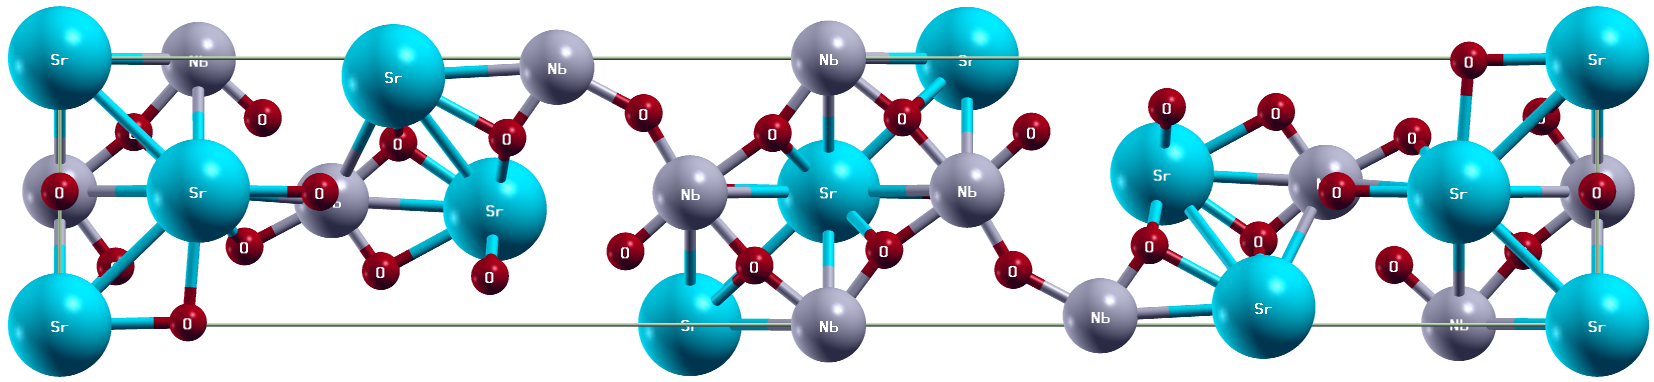
\includegraphics[width=200pt]{graph/pwi2xsf.png}}
  \caption{Struktur kristal $\mathrm{SrNbO_{3,4}}$. Atom Sr ditandai warna biru, atom Nb ditandai warna abu-abu, atom O ditandai warna merah. Terdapat jarak yang renggang dan membentuk 3 grup (kiri, tengah, kanan) karena adanya tambahan atom oksigen.}
\end{figure}

Kami memodelkan sistem material $\mathrm{SrNbO_{3,4}}$ dengan persamaan hamiltonian Tight-Binding multiband,
$$ H_{ij}(\vec{k}) = \frac{1}{N}\sum_{nm}\sum_{\alpha \beta}e^{-i\vec{k} \cdot (\vec{r}_{in}-\vec{r}_{jm})} t_{in\alpha, jm\beta} $$
dengan asumsi elektron hopping dari orbital $i$ ke $j$, atom $n$ ke $m$, dan unit cell $\alpha$ ke $\beta$ sebanyak N unit cell. Posisi elektron di orbital $i$ dan atom $n$ berada di $r_{in}$, dan elektron di orbital $j$ dan atom $m$ berada di $r_{jm}$. Momentum yang dimiliki elektron sebesar $\vec{k}$. Sedangkan $t_{in\alpha, jm\beta}$ merupakan parameter hopping pada elektron.

Dalam tulisan kali ini, kami memodelkan material tersebut dengan beberapa jenis orbital yang dianggap sebagai elektron valensi. Seperti atom Strontium (Sr) memiliki orbital $4s-5s-4p-5p$, atom Niobium (Nb) memiliki orbital $4s-5s-4p-5p-4d$, dan atom Oksigen (O) memiliki orbital $2s-2p$. Material yang kami gunakan memiliki 10 atom Strontium, 10 atom Niobium, dan 34 atom Oksigen\cite{persson}. Sehingga terdapat 346 jenis orbital elektron valensi yang kami gunakan.

\section{METHOD}
Pada tahap awal, kami melakukan perhitungan secara first-principle dengan menghitung density functional theory (DFT) dan maximally-localised wannier function (MLWF). Untuk perhitungan DFT, kami menggunakan package Quantum Espresso\cite{QE-2017,QE-2009}. Sedangkan untuk perhitungan MLWF, kami menggunakan package Wannier90\cite{wannier}. Perhitungan DFT dilakukan untuk mendapatkan electronic structure secara lengkap dari semua orbital valensi setiap atom. Selanjutnya dari hasil perhitungan tersebut, dilanjutkan denganperhitungan MLWF untuk mendapatkan parameter tight-binding. Dari parameter tersebut akan kami gunakan untuk mengkonstruksi matriks hamiltonian tight-binding multiband.

Dari matriks hamiltonian tight-binding tersebut, kami melakukan perhitungan eigenvalues untuk mendapatkan band-structure dengan pendekatan tight-binding. dan perhitungan rapat elektron dengan menggunakan green function. Persamaan green function yang digunakan adalah,
$$ [G(\omega, \vec{k})] = \frac{1}{(\omega + i\eta)[I] - [H(\vec{k})]} $$
Dari green function tersebut dapat digunakan untuk menentukan partial density of states (PDOS) dengan menggunakan,
$$ PDOS_\alpha(\omega) = -\frac{1}{\pi}Im\sum_k{[G_{\alpha \alpha}(\omega, \vec{k})]} $$
dan juga total density of states (DOS) dengan menggunakan,
$$ DOS (\omega) = \sum_\alpha{PDOS_\alpha(\omega)}$$


\section{RESULT AND DISCUSSION}
\begin{figure}[h]
  \centerline{\includegraphics[width=200pt,angle=-90]{graph/band_dos_qe_23x3x17.eps}}
  \caption{Band Structure and Density of States from First Principle Calculation Using Quantum Espresso}
\end{figure}

Perhitungan first-principle pada material $\mathrm{SrNbO_{3,4}}$ menghasilkan grafik struktur pita energi yang memiliki struktur anisotropik. Dapat dilihat pada gambar 2 bahwa untuk arah sumbu a ($\mathrm{X - \Gamma}$) memiliki sifat konduktor, sedangkan untuk arah sumbu b ($\mathrm{\Gamma - Y}$) dan c ($\mathrm{\Gamma-Z}$) memiliki sifat insulator. Pada perhitungan tersebut, besar dari fermi level diatur berdasarkan data eksperimen dari angular-resolved photoemission spectroscopy (ARPES)\cite{kuntscher}.

Hasil perhitungan dengan pendekatan tight-binding menunjukkan bahwa band-structure pada gambar 3 sama seperti perhitungan first-principle. Sama halnya dengan rapat keadaan pada gambar 4 menunjukkan bahwa hasil perhitungan dengan pendekatan tight-binding dan first principle sama. Hal tersebut menunjukkan bahwa hanya dengan model pendekatan tight-binding saja sudah cukup untuk dapat menghasilkan sifat fisis yang sama sesuai dengan perhitungan first-principle.

\begin{figure}[b]
  \centerline{\includegraphics[width=200pt]{graph/band_TB_original.eps}}
  \caption{Band Structure from Hamiltonian Tight-Binding Multiband.}
\end{figure}

Kami mereduksi matriks hamiltonian tight binding dengan cara menghilangkan orbital-orbital yang tidak memiliki kontribusi di rentang energi 3 hingga 13.5 eV. Karena di rentang energi tersebut terdapat banyak elektron yang menempati keadaan tersebut, dan juga rentang energi tersebut terletak di sekitar fermi level. Untuk melihat orbital mana saja yang tidak memiliki kontribusi di rentang energi tersebut, kami menggunakan perhitungan partial density of states (PDOS) untuk setiap orbital dan menghilangkan orbital yang memiliki nilai rendah di rentang energi tersebut.

Dari 346 orbital elektron valensi, kami mereduksi 133 orbital yang tidak memiliki kontribusi elektron di rentang frekuensi tersebut. Hasil dari band structure setelah orbital tersebut direduksi dapat dilihat pada gambar 5. Pada gambar tersebut dapat dilihat bahwa material tersebut tetap dapat mempertahankan karakteristik anisotropik seperti sebelumnya.

\begin{figure}[h]
  \centerline{\includegraphics[width=200pt]{graph/dos_qetb.eps}}
  \caption{Comparison Density of States between First Principle Calculation and Tight Binding Calculations.}
\end{figure}

Berdasarkan perhitungan PDOS dengan DFT menunjukkan bahwa di sekitar fermi level didominasi oleh orbital-d pada atom Nb\cite{Wan2017}. Dan juga pada reduksi hamiltonian tight-binding sebelumnya didapat bahwa terdapat beberapa atom Nb yang mana orbital-d nya mendominasi di daerah sekitar fermi level. Atom Nb tersebut berada di batas-batas grup yang terbentuk karena adanya tambahan oksigen dari $\mathrm{SrNbO_{3}}$ menjadi $\mathrm{SrNbO_{3,4}}$ (fig 1). Selain itu, beberapa atom oksigen yang berada di antara atom Nb juga memiliki konstribusi di sekitar fermi level.

Kami belum dapat mereduksi lebih dari 133 orbital dikarenakan apabila lebih dari orbital tersebut direduksi, maka struktur pita yang membuat karakteristik material menjadi anistropik akan runtuh. Sehingga dapat dikatakan bahwa selain kontribusi atom Nb dan O yang telah dijelaskan sebelumnya, struktur kristal $\mathrm{SrNbO_{3,4}}$ itu sendiri juga memiliki kontribusi yang kuat atas sifatnya yang anisotropik.

\begin{figure}[b]
  \centerline{\includegraphics[width=200pt]{graph/TB_bands.eps}}
  \caption{Band Structure after Orbitals Reduction.}
\end{figure}

\section{CONCLUSION}
Kami telah menjelaskan tentang materials $\mathrm{SrNbO_{3,4}}$ yang memiliki karakteristik anisotropik dengan menggunakan pendekatan tight-binding. Untuk mengetahui orbital mana saja yang berkontribusi atas karakterisknya yang anisotropik, kami mereduksi orbital yang tidak berkontribusi di rentang frekuensi $3-13.5 eV$. Kami menemukan bahwa orbital-d pada atom Nb yang berada di batas grup, atom O yang berada di antara atom Nb, dan struktur kristal $\mathrm{SrNbO_{3,4}}$ itu sendiri yang membuat material tersebut memiliki karakteristik anisotropik.

% Sections that will go in second font

% Acknowledgement
\section{ACKNOWLEDGMENTS}
The computation in this work has been done using the facilities of HPC LIPI,
Indonesian Institute of Sciences (LIPI)

% References

\nocite{*}
\bibliographystyle{unsrt}%
\bibliography{workspace}%


\end{document}